\chapter{The Role of Croup Communication}
The membership of groups can be created in different ways, in replication circumstances, there is a strong requirement for dynamic membership. A group membership service implements several features:
\begin{itemize}
    \item Provides an interface to manage group
    \item Implement a fault detector
    \item Notifies the group changes to the group members
    \item Makes the group address expansion
\end{itemize}

A group membership service maintains group views, which are lists of the current group members, identified by their unique process identifiers. For each group \(g\) the group service delivers to any member process \(p \in g\) a series of views. In general, a member \textit{delivering a view}, when a membership change occurs and the application is notified of the new membership.
Some basic requirements for \textbf{view delivery} are as follows:
\begin{itemize}
    \item \textbf{Order:} if a process \(p\) delivers view \(v(g)\) and then \(v'(g)\), then no other process \(q  \neq p\) delivers \(v'(g)\) before \(v(g)\)
    \item \textbf{Integrity:} if a process \(p\) delivers view \(v(g)\), then \(p \in v(g)\)
    \item \textbf{Non-triviality:} if process \(q\) joins a group and is or becomes indefinitely reachable from process \(p \neq q\)
\end{itemize}

\begin{figure}[!h]
    \centering
    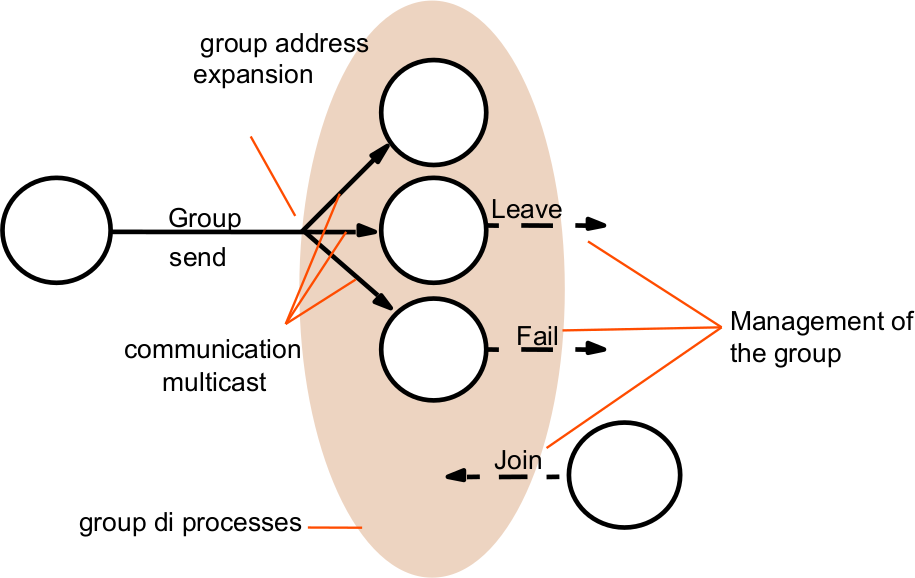
\includegraphics[width=.60\linewidth]{images/roleGroupCommunication/GroupOfProcesses.png}
    \caption{Services for a group of processes}
\end{figure}
\newpage

A \textbf{view-synchronous} group communication system makes \textbf{additional guarantees} to those above about the delivery ordering of view notifications with respect to the delivery of multicast messages. These guarantees are:
\begin{itemize}
    \item \textbf{Agreement:} correct processes deliver the same sequence of views and the same set of messages in any given view
    \item \textbf{Integrity:} if a correct process \(p\) delivers message \(m\), then it will not deliver \(m\) again
    \item \textbf{Validity:} correct processes always deliver the messages that they send. If a process \(q\) has not delivered a message, system notifies and successive views exclude \(q\)
\end{itemize}

Considering the following image, a group with three processes, \(p\), \(q\) and \(r\)
\begin{itemize}
    \item \textbf{Picture (a):} suppose that \(p\) sends a message \(m\) while in view (\(p\), \(q\), \(r\)) but that \(p\) crashes soon after sending \(m\), while \(q\) and \(r\) are correct. One possibility is that \(p\) crashes before \(m\) has reached any other process. In this case, \(q\) and \(r\) each deliver the new view (\(q\), \(r\)), but neither ever delivers \(m\)
    \item \textbf{Picture (b):} the other possibility is that \(m\) has reached at least one of the two surviving processes when \(p\) crashes. Then \(q\) and \(r\) both deliver first \(m\) and then the view (\(q\), \(r\)) 
    \item \textbf{Picture (c):} it is not allowed for \(q\) and \(r\) to deliver first the view (\(q\), \(r\)) and then \(m\)
    \item \textbf{Picture (d):} since then they would deliver a message from a process that they have been informed has failed, nor can the two deliver the message and the new view in opposite orders
\end{itemize}

\begin{figure}[!h]
    \centering
    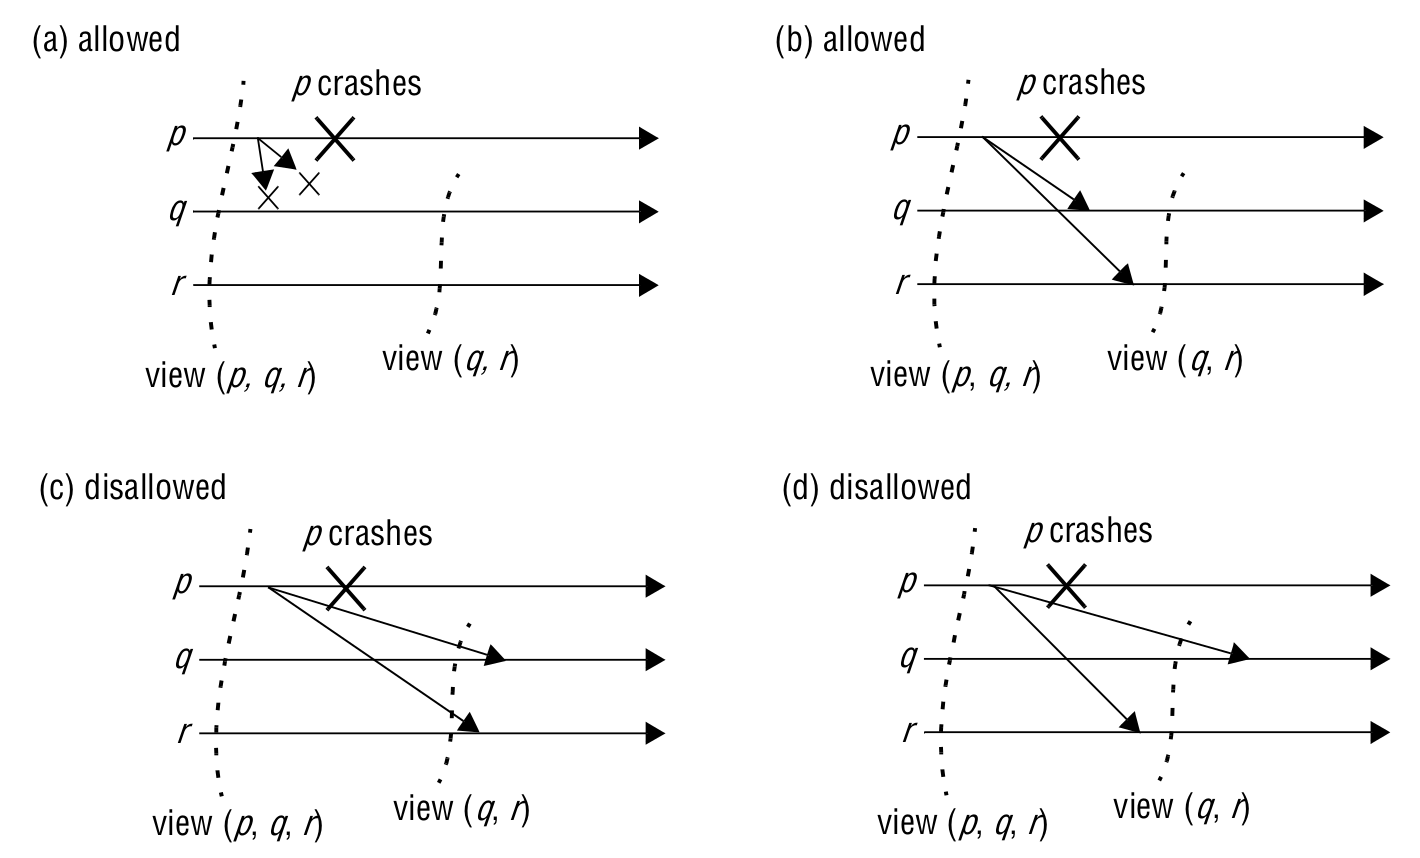
\includegraphics[width=.70\linewidth]{images/roleGroupCommunication/ConsistentMessage.png}
    \caption{Delivery of consistent messages}
\end{figure}
\newpage

\section{Fault-tolerant services}
In the following pages we will examine how to provide a service that is correct, despite process failures, by replicating data and functionality at replica managers.

\subsection{Passive replication}
In this model at any time there is a \textbf{primary replica} manager and one or more \textbf{secondary} replica managers. So \textit{front ends} communicate only with the primary replica manager to obtain the service. The primary replica manager executes the operations and sends copies of the updated data to the backups. If the primary fails, one of the backups is promoted to act as the primary. The sequence of events when a client requests an operation to be performed is as follows:
\begin{itemize}
    \item \textbf{Request:} the front end issues the request, containing a unique identifier, to the primary replica manager
    \item \textbf{Coordination:} the primary takes each request atomically, in the order in which it receives it
    \item \textbf{Execution:} the primary executes the request and stores the response.
    \item \textbf{Agreement:} if the request is an update, then the primary sends the updated state
    \item \textbf{Response:} the primary responds to the front end, which hands the response back to the client
\end{itemize}

\begin{figure}[!h]
    \centering
    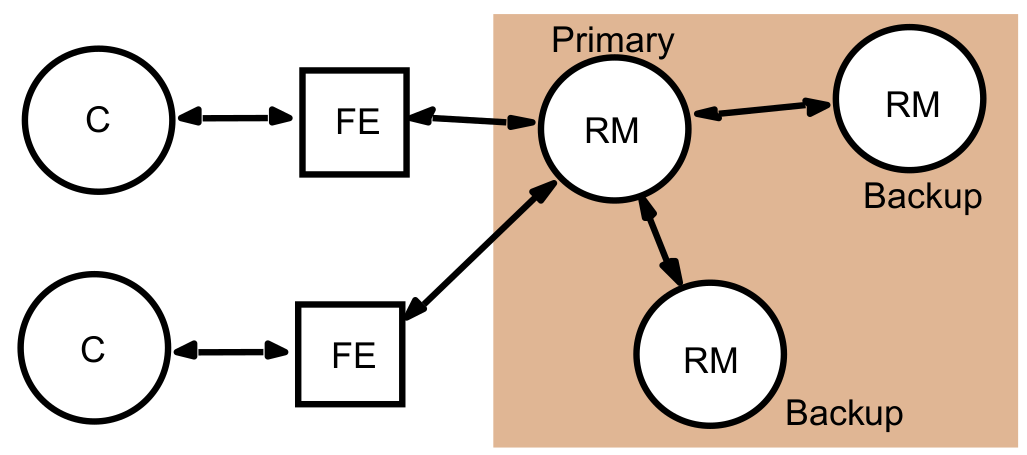
\includegraphics[width=.70\linewidth]{images/roleGroupCommunication/PassiveModel.png}
    \caption{The passive model}
\end{figure}
\newpage

This system obviously implements linearizability if the primary is correct, since the primary sequences all the operations upon the shared objects. In other words, if the primary fails another backup is used to substitute it. That is if:
\begin{itemize}
    \item The primary is replaced by a unique backup
    \item The replica managers that survive agree on which operations had been performed
\end{itemize}

\section{Active replication}
In the \textbf{active model} of replication for fault tolerance, the replica managers are state machines that play equivalent roles and are organized as a group.

If any replica manager crashes, this need have no impact upon the performance of the service, since the remaining replica managers continue to respond in the normal way. Under active replication, the sequence of events when a client requests an operation to be performed is as follows:
\begin{itemize}
    \item \textbf{Request:} the front end attaches a unique identifier to the request and multicasts it to the group of replica managers, using a totally ordered, reliable multicast primitive
    \item \textbf{Coordination:} the group communication system delivers the request to every correct replica
    \item \textbf{Execution:} every replica manager executes the request
    \item \textbf{Agreement:} no agreement phase is needed, because of the multicast delivery semantics.
    \item \textbf{Response:} each replica manager sends its response to the front end. The number of replies that the front end collects depends upon the failure assumptions and the multicast algorithm
\end{itemize}

\begin{figure}[!h]
    \centering
    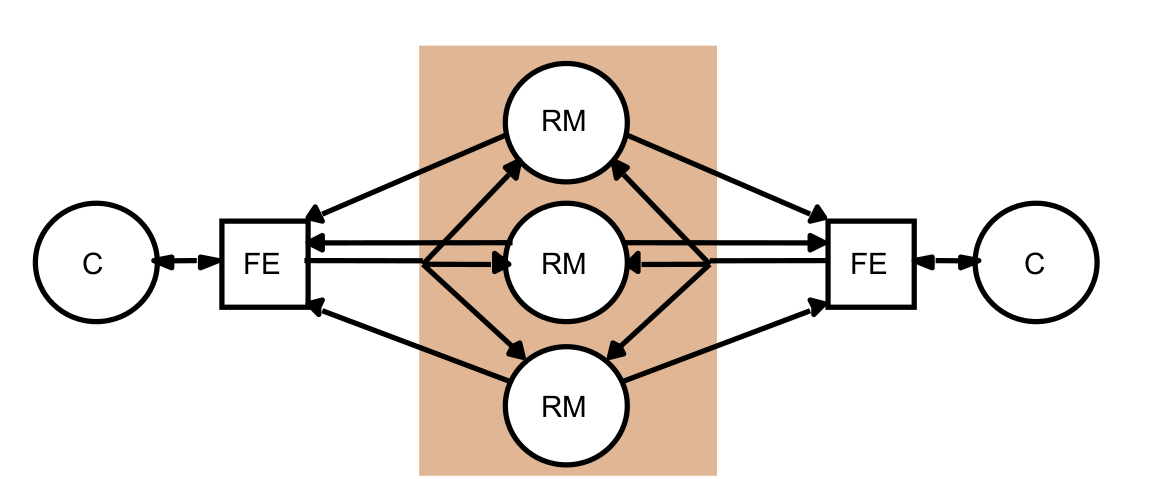
\includegraphics[width=.70\linewidth]{images/roleGroupCommunication/ActiveReplication.png}
    \caption{ The active replication model}
\end{figure}

\section{High available services}
Now we consider how to apply \textbf{replication techniques} to make services highly available. Our attention now is on giving clients access to the service for as much of the time as possible.

\subsection{The Gossip Architecture}
Gossip architecture was developed as a framework for implementing \textit{highly available services} by \textbf{replicating data} close to the points where groups of clients need it. The name reflects the fact that the \textbf{replica managers} exchange "gossip" messages periodically in order to \textit{transport the updates} they have each received from clients.

\begin{figure}[!h]
    \centering
    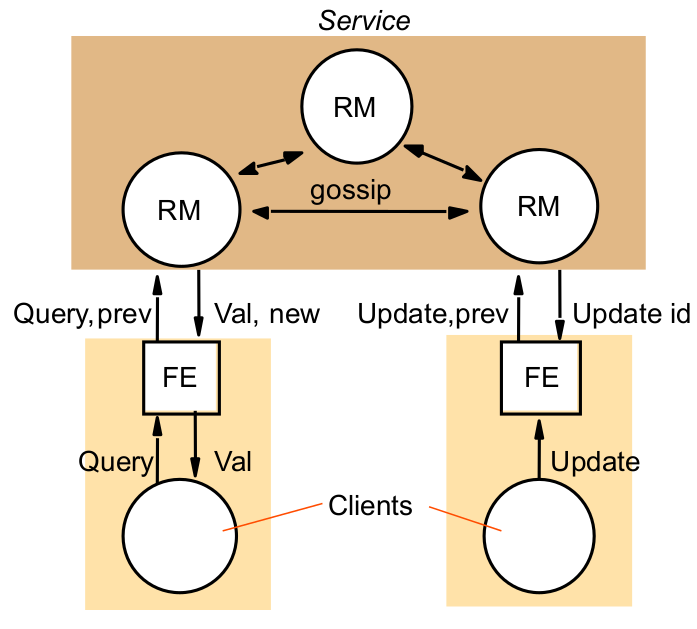
\includegraphics[width=.60\linewidth]{images/roleGroupCommunication/GossipService.png}
    \caption{Query and update operations in a gossip service}
\end{figure}

A gossip service provides two basic types of operations:
\begin{enumerate}
    \item \textit{Queries:} read-only operations
    \item \textit{Updates:} modify but not read
\end{enumerate}
The system makes two guarantees:
\begin{itemize}
    \item \textit{Each client obtains a consistent service over time}
    \item \textbf{Relaxed consistency between replicas}
\end{itemize}

\textbf{The front end’s version timestamp.} In order to control the ordering of operation processing, each front end keeps a \textbf{vector timestamp} that reflects the version of the \textit{latest data values} accessed by the front end.
\begin{itemize}
    \item It contains an entry for every replica manager
    \item The front end sends it in every request message to a replica manager, together with a description of the query or update operation itself
    \item When a replica manager returns a value as a result of a query operation, it supplies a new vector timestamp, since the replicas may have been updated since the last operation
    \item An update operation returns a vector timestamp that is unique to the update.
    \item Each returned timestamp is merged with the front end’s previous timestamp to record the version of the replicated data that has been observed by the client.
\end{itemize}

\begin{figure}[!h]
    \centering
    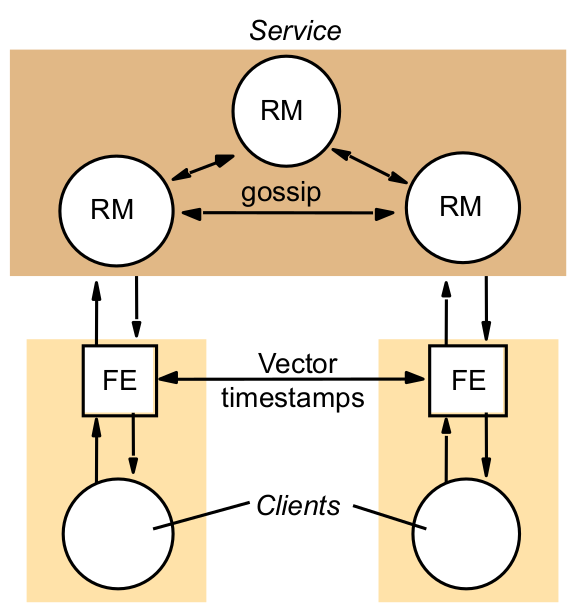
\includegraphics[width=.60\linewidth]{images/roleGroupCommunication/GossipArchitectureTimestamp.png}
    \caption{Front ends propagate their timestamps whenever clients communicate directly}
\end{figure}

\textbf{Replica manager state.} Regardless of the application, if contains the following steps:
\begin{itemize}
    \item \textbf{Value:} this is the value of the application state as maintained by the replica manager
    \item \textbf{Value timestamp:} this is the vector timestamp that represents the updates that are reflected in the value
    \item \textbf{Update log:} all update operations are recorded in this log as soon as they are received 
    \item \textbf{Replica timestamp:} this vector timestamp represents those updates that have been accepted by the replica manager
    \item \textbf{Executed operation table:} to prevent an update being applied twice, the "executed operation" table is kept, containing the unique front-end-supplied identifiers of updates that have been applied to the value
    \item \textbf{Timestamp table:} this table contains a vector timestamp for each other replica manager, filled with timestamps that arrive from them in gossip messages
\end{itemize}

\section{Transactions with replicated data}
A \textbf{transaction} on replicated objects should \textbf{appear the same} as one with \textit{non-replicated} objects, and the \textbf{effect} should be the the \textit{same} as if they had been performed one at a time on a \textit{single set of objects}. This propriety is called \textbf{one-copy serializability}.

The implementation of \textit{one-copy serializability} is illustrated by \textit{read-one/write-all}, a simple replication scheme in which \textit{read} operations are performed by a single replica manager and \textit{write} operations are performed by all of them.

\subsection{Architectures for replicated transactions}
A front end may either multicast client requests to groups of replica managers or send each request to a single replica manager. The replica manager that receives a request to perform an operation on a particular object is responsible for getting the cooperation of the other replica managers in the group that have copies of that object. For example, in the \textit{read-one/write-all} scheme, a \textit{read} request can be performed by a \textbf{single replica manager}, whereas a \textit{write} request must be performed by \textit{all the replica managers} in the group.

\begin{figure}[!h]
    \centering
    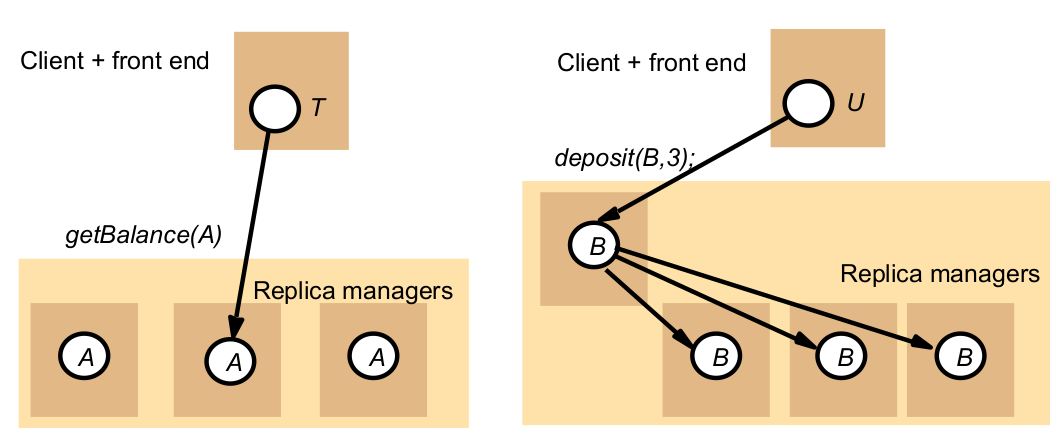
\includegraphics[width=.70\linewidth]{images/roleGroupCommunication/TransactionsOnReplicatedData.png}
    \caption{Transactions on replicated data}
\end{figure}

\subsection{Available copies replication}
Simple \textit{read-one/write-all} replication is not a realistic scheme. The \textbf{available copies} scheme is designed to allow for some replica managers being temporarily unavailable. \textit{Read} requests can be performed by the replica manager that receives them. write requests are performed by the receiving replica manager and all the other available replica managers in the group. For example the bellow image:
\begin{itemize}
    \item \textit{getbalance} operation of transaction \(T\) is performed by \(X\)
    \item Whereas its \textit{deposit} is performed by \(M\), \(N\) and \(P\).
    \item Concurrency control at each replica manager affects the operations performed locally
    \item At \(X\), transaction \(T\) has read \(A\) and therefore transaction \(U\) is not allowed to update \(A\) with \textit{deposit} operation until transaction \(T\) has completed
\end{itemize}

\begin{figure}[!h]
    \centering
    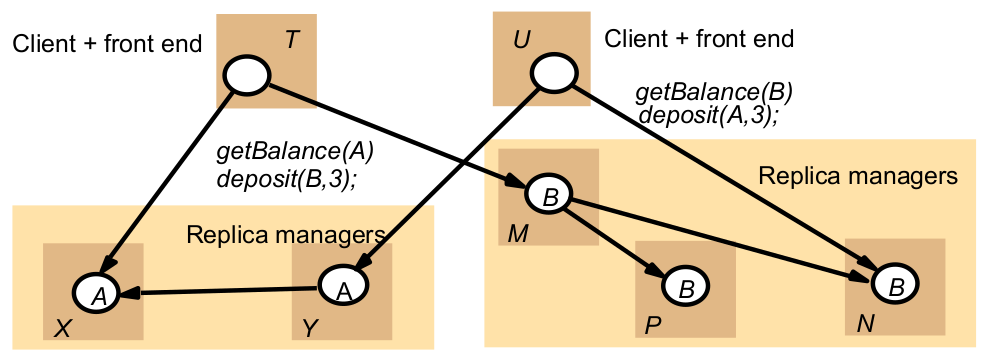
\includegraphics[width=.70\linewidth]{images/roleGroupCommunication/AvailableCopies.png}
    \caption{Available copies}
\end{figure}

\section{Network partitions}
A network partition separates a group of replica managers into two or more subgroups in such a way that the members of one subgroup can communicate with one another but members of different subgroups cannot communicate with one another.

In the following image, the replica managers receiving the deposit request cannot send it to the replica managers receiving the withdraw request. Replication schemes are designed with the assumption that partitions will eventually be repaired. 
\begin{figure}[!h]
    \centering
    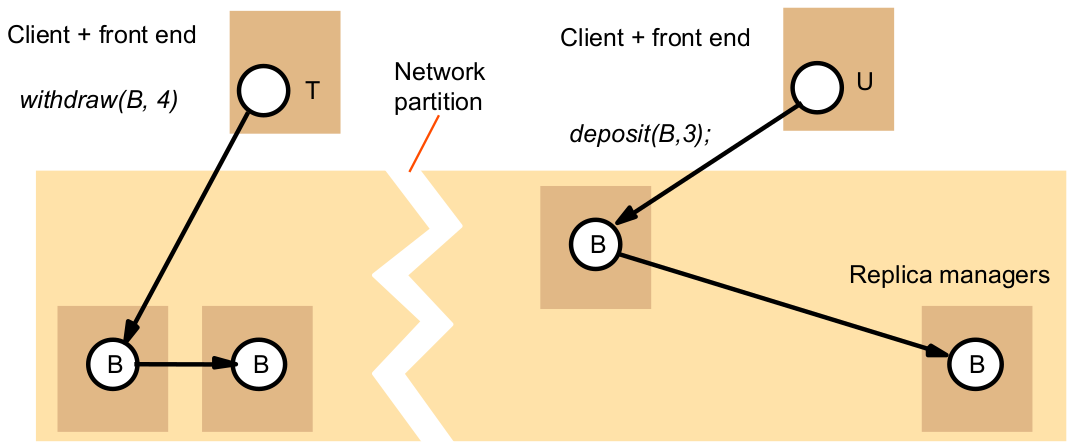
\includegraphics[width=.70\linewidth]{images/roleGroupCommunication/NetworkPartition.png}
    \caption{Network partition}
\end{figure}
\newpage
The optimistic schemes do not limit availability during a partition, whereas pessimistic schemes do.
\begin{itemize}
    \item The \textbf{optimistic approach} allows updates in all partitions
    \item The \textbf{pessimistic approach} limits availability even when there are no partitions, but it prevents any inconsistencies occurring during partitions. In other words it is based on the idea of \textbf{quorum}, only the partition that satisfy the quorum is available to the client.
    \item The \textbf{Combined approach} is based on algorithm of \textbf{virtual partition}
\end{itemize}



\subsection{Virtual Partition}
A \textbf{virtual partition} is an abstraction of a real partition and contains a set of replica managers.
Note that:
\begin{itemize}
    \item \textit{"network partition"} refers to the \textbf{barrier} that divides replica managers into several parts
    \item \textit{"virtual partition"} refers to the parts themselves
\end{itemize}

\begin{figure}[!h]
    \centering
    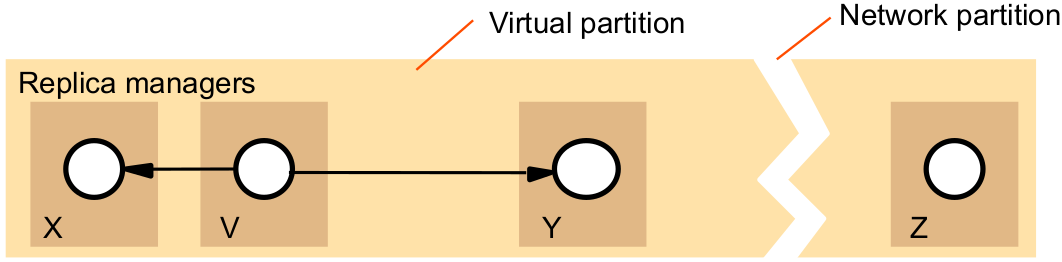
\includegraphics[width=.70\linewidth]{images/roleGroupCommunication/VirtualPartition.png}
    \caption{Virtual partition}
\end{figure}

\subsection{Creating a virtual partition}
\begin{enumerate}
    \item Phase
    \begin{itemize}
        \item The initiator sends a \textbf{Join} request to each potential member. The argument of \textit{Join} is a \textbf{proposed logical timestamp} for the new virtual partition
        \item When a replica manager receives a \textbf{Join} request, it \textbf{compares} the proposed logical timestamp with that of its current virtual partition
        \begin{itemize}
            \item If the proposed logical timestamp is greater it agrees to join and replies \textbf{Yes}
            \item If it is less, it refuses to join and replies \textbf{No}
        \end{itemize}
    \end{itemize}
    \item Phase
    \begin{itemize}
        \item If the initiator has received \textbf{sufficient} \textit{Yes} replies to have read and write quora, it may complete the \textbf{creation of the new virtual partition} by sending a \textit{Confirmation} message to the sites that agreed to join. The creation timestamp and list of actual members are sent as arguments
        \item Replica managers receiving the \textit{Confirmation} message join the new virtual partition and record its creation timestamp and list of actual members
    \end{itemize}
\end{enumerate}

In summary:
\begin{itemize}
    \item  When a replica manager receives a request it tries to create a virtual partition as large as possible in order to reach the quorum
    \item Replica managers can communicate using an alternative way
    \item This strategy improves the availability since the virtual partition can be greater than the real one on the network
\end{itemize}